\documentclass[11pt]{article}
\usepackage{setspace}
\usepackage[a4paper,margin=1in]{geometry}
\geometry{margin=0.85in}
\setstretch{1.0}
\usepackage{graphicx}
\usepackage{array}
\usepackage{setspace}
\usepackage{parskip}
\usepackage{ragged2e}

\pagestyle{empty}
\setstretch{1.05}

\begin{document}


% Title
\begin{center}
    {\Large \textbf{Job Application}} \\[3cm]
    
    {\Huge \textbf{Zhongli Wang}} \\[0.4cm]
    
    {\LARGE Application for Business Data Analyst}
\end{center}

\vspace{0.6cm}

% Large picture in the middle
\begin{center}
    \IfFileExists{../zhongli-wang-profile.jpg}{
        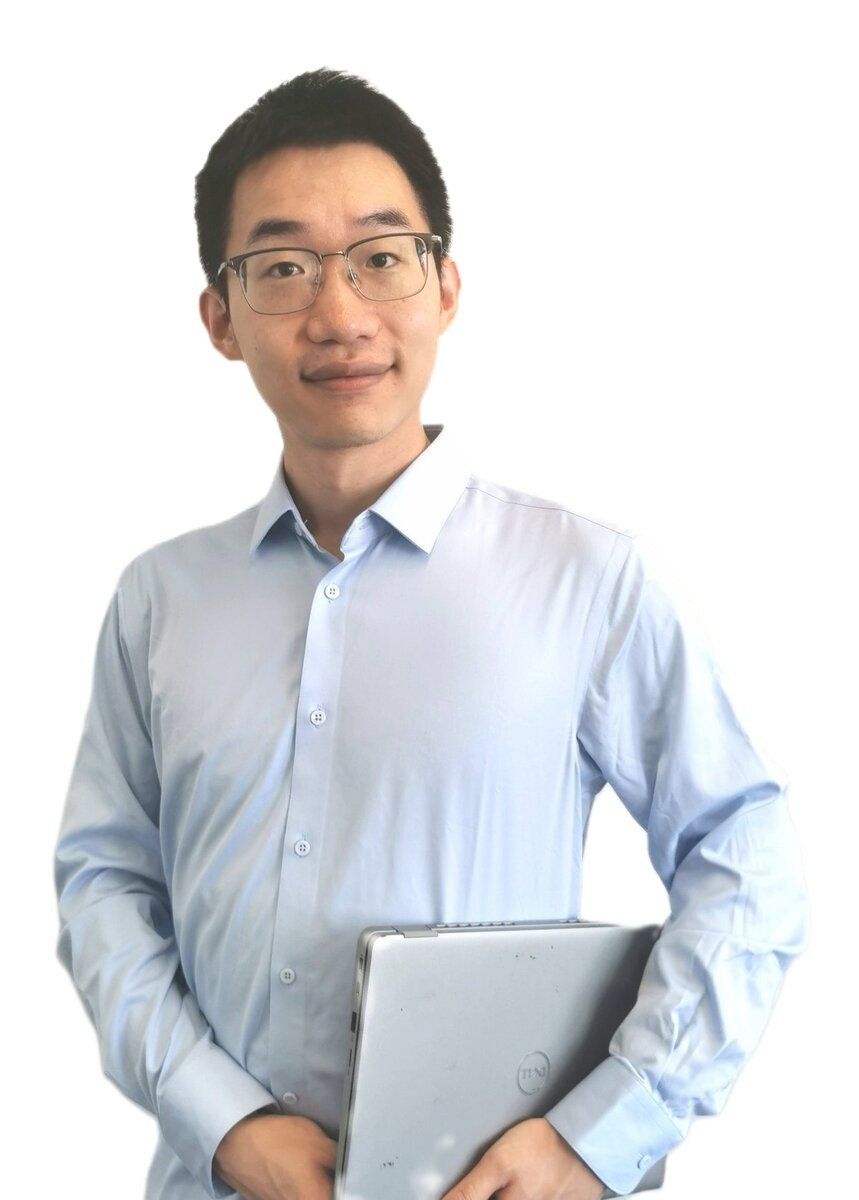
\includegraphics[
            width=0.55\textwidth,
            height=0.45\textheight,
            keepaspectratio
        ]{../zhongli-wang-profile.jpg}
    }{
        \vspace{0.45\textheight}
    }
\end{center}

\vspace{0.7cm}

% \vspace{3cm}


% Personal details
\begin{center}
\renewcommand{\arraystretch}{1.35}
\begin{tabular}{>{\bfseries}p{4.2cm} p{8.5cm}}


Address: & Astastrasse 22, 33617 Bielefeld, Germany \\

Number: & +49 160 9541 6015 \\

Email: & nkwangzhongli@gmail.com \\
\end{tabular}
\end{center}

\vfill

% \begin{center}
%     \small Last updated: \today
% \end{center}
\newpage
\enlargethispage{4\baselineskip}

\begin{flushright}
Zhongli Wang \\
Astastrasse 22 \\
33617 Bielefeld\\
Germany \\
\end{flushright}

\vspace{0.1cm}

\vspace{0.1cm}

\noindent
CBRE Group, Inc. \\
GWS Segment \\
Hong Kong SAR

\vspace{0.12cm}

\noindent
\textbf{Application for Business Data Analyst (Job ID 302816)}

\vspace{0.1cm}

\noindent Dear CBRE recruiting team,

I recently completed my Ph.D. in Economics in a joint program between Bielefeld University and UCSC Milan,
successfully defending my dissertation on September 21, 2026.
I also hold an M.A. in Business and Economics with a major in Banking and Finance and a minor in Data Science.
My doctoral research applies computational and econometric methods to questions of firm behavior,
research and development investment, and industrial market dynamics,
providing a strong foundation for turning complex data into accurate metrics and actionable business intelligence.

I am particularly drawn to CBRE as the world's largest commercial real estate services and investment firm,
where the Data Science \& Analytics function directly shapes business decisions across the GWS segment.
The role's focus on data collection, auditing, and accurate key metric reporting matches the rigor of my academic training,
while the mandate to develop data models, reporting systems, automation tools, and dashboards
aligns closely with the technical toolkit I have built across my studies and research.
My research approach mirrors what the role demands:
clean and validate data carefully, analyze it with appropriate quantitative methods,
and communicate complex findings logically and concisely to stakeholders.
My relevant experience comprises:

\begin{itemize}
    \item \textbf{Data analysis and reporting:} I have extensive experience collecting, cleaning, auditing, and analyzing large-scale datasets to answer concrete business and research questions. My doctoral research develops quantitative models of firm investment and market outcomes, and in published work I applied machine learning methods (XGBoost, Random Forest) to high-dimensional data to identify patterns and predict outcomes.
    \item \textbf{Dashboards, automation, and visualization:} I work fluently with Python, R, and Stata to build reproducible data pipelines, automated reporting workflows, and clear visualizations. At the University of Zurich I worked on SYLVA, a system that automated grading workflows, giving me first-hand experience in automating processes and improving reporting efficiency. I regularly prepare reports and presentations that translate technical results for non-technical audiences.
\end{itemize}

As a native Mandarin Chinese speaker with excellent command of English and German at C1 level,
I am confident communicating with stakeholders, management, and vendors across CBRE's international teams in Hong Kong and beyond.
I am highly motivated to apply my analytical skills and inquisitive mindset to CBRE's data-driven decision-making,
and I am willing to relocate to Hong Kong.
I am also approved under Hong Kong's Top Talent Pass Scheme (TTPS), so I am fully authorized to live and work in Hong Kong without sponsorship.

Thank you so much for considering my application!
I would welcome the opportunity to discuss how my background and abilities could contribute to CBRE's data and analytics work.
Should it better suit your team's needs, I would also be happy to begin in an internship capacity.

\vspace{0.08cm}
\noindent Kind regards, \\
% \vspace{0.1cm}
\noindent
\includegraphics[width=2.7cm,keepaspectratio]{../Wang-sig.jpg} \\
\noindent Zhongli Wang


\end{document}
